\input sys/inputs.tex

\usepackage{tikz}

\begin{document}

\bigheading{Plakáty Kabátů}

% \info{task_name}{infile}{outfile}{points}{timelimit}{memlimit}
% leave this values, if you are not interested
\info{posters}{stdin}{stdout}{100}{2000 ms}{1 GB}

Mirek je kromě jiného také zažraným fanouškem Kabátů.
Účastní se všech jejich konzertů a sbírá jejich plakáty.
Pokaždé, když získá nový plakát, tak si ho pověsí na zeď nad postel.
Po mnoha letech sbírání plakátů Kabátů jimi má pokrytou téměř celou zeď
a už nemůže najít žádné místo na nové.
Zrovna ale dostal nové kousky do své sbírky a potřebuje pro ně najít nejlepší místo.
Pro každý nový plakát by chtěl Mirek vědět, jak moc bude překrývat ostatní plakáty.

\heading{Úloha}

Jsou zadány souřadnice plakátů, které již na stěně visí.
Dále dostanete souřadnice, kam se budou věšet nové plakáty.
Pro každý nový plakát, nalezněte souhrnný obsah plakátů, které by nový plakát zakryl, pokud by byl skutečně pověšen.

Plakáty visící na stěně se mohou překrývat a pokud je jejich průnik pokryt, tak tuto společnou část nezapočítávejte dvakrát.

\heading{Vstup}

Na prvním řádku vstupu vypište jedno celé číslo $N$ ($1 \le N \le 100\,000$)
-- počet plakátů, které již na stěně visí.
Na následujících $N$ řádcích naleznete popis těchto plakátů.
Na $(N+2)$-hém řádku je jedno celé číslo $M$ ($1 \le M \le 100\,000$)
-- počet plakátů, které Mirek teprve plánuje pověsit na zeď.
Vstup končí $M$ řádkami, které popisují tyto plakáty.

Každý plakát si můžete představit jako obdélník, jehož hrany jsou rovnoběžné s osami souřadnicové sítě.
Tento obdélník je popsán čtyřmi celými čísly $x_1$, $y_1$, $x_2$, $y_2$
($0 \le x_1 < x_2 \le 10^9$, $0 \le y_1 < y_2 \le 10^9$),
vyjadřujícími souřadnice levého dolního rohu a pravého horního rohu plakátu.

Ve $12.5\%$ vstupů platí, že $n, m \le 10$, souřanice nejsou větší než $100$.

Ve $25\%$ vstupů navíc platí, že $n, m \le 50$.

V $50\%$ vstupů platí, že $n, m \le 1000$.

V $50\%$ vstupů souřadnice nejsou větší než $30\,000$.

\heading{Výstup}

Pro každý nový plakát vypište jedno celé číslo -- odpověď na Mirkovu otázku.
Odpovědi musíte vypsat ve stejném pořadí, ve kterém byly plakáty zadány na vstupu.

\newpage

\heading{Příklad}


\sampleIN
2
0 1 3 5
2 3 6 6
2
1 0 5 4
4 2 7 7
\sampleCOMMENT
Mirkova zeď vypadá tak, jako na následujícím obrázku.
Čárkované obdélníky reprezentují nové plakáty, zatímco obdélníky,
jejiž obvod je tvořen plnou čarou,
reprezentují plakáty, které na zdi již visely.
\begin{center}
	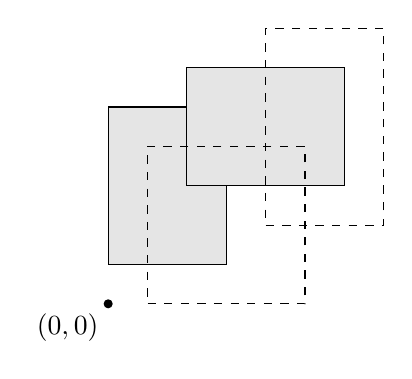
\begin{tikzpicture}[scale=0.5]
		\filldraw (0, 0) node[below left] {$(0, 0)$} circle(0.1);
		\filldraw[gray!20] (0, 1) -- (3, 1) -- (3, 5) -- (0, 5) -- cycle;
		\draw (0, 1) -- (3, 1) -- (3, 5) -- (0, 5) -- cycle;
		\filldraw[gray!20] (2, 3) -- (6, 3) -- (6, 6) -- (2, 6) -- cycle;
		\draw (2, 3) -- (6, 3) -- (6, 6) -- (2, 6) -- cycle;
		\draw[dashed] (1, 0) -- (5, 0) -- (5, 4) -- (1, 4) -- cycle;
		\draw[dashed] (4, 2) -- (7, 2) -- (7, 7) -- (4, 7) -- cycle;
	\end{tikzpicture}
\end{center}
\sampleOUT
8
6
\sampleCOMMENT
\sampleEND


\end{document}
